%!TEX root = ../thesis.tex

% \vspace{-1pt}

\section{本章の概要}
本章では,移動ロボットのナビゲーションで予測結果を利用する実験を行い,その結果を評価する.まず,実験の概要と方法について説明し,次に実験シナリオと使用したシミュレータ環境について述べる.最後に,実験結果を基に考察を行う.

\section{実験概要}
予測結果をナビゲーションに応用したシステムによって,移動ロボットの挙動がどのように変化するか観察し,評価するために実験を行う.実験では,2つのナビゲーションシナリオで移動ロボットを自律走行させてデータを取得した.なお,各シナリオごとに10回走行させた.

\section{実験方法}
実験の予測は,\ref{chap:proposed_method}章のネットワークを用いて行った.しかし,使用したモデルに関しては,ホールドアウト(Hold Out)方式で学習を行った.それ以外は,同様の学習条件である.
また,\ref{chap:application}章で述べたシステムを用いてナビゲーションに予測結果を応用している.

実験は\figref{Fig:sim-env}に示すような,Gazebo\cite{Gazebo62:online}のシミュレータ環境で行う.また,\figref{Fig:sim-robot}に示すように,シミュレータで再現した移動ロボット(ORNE-box2\cite{井口颯人2023屋外自律移動ロボットプラットフォーム-orne})を使用した.\figref{Fig:sim-actor}に示す歩行者は,Gazeboのプラグイン\cite{Actors-G87:online}を使用している.

\begin{figure}[H]
  \centering
 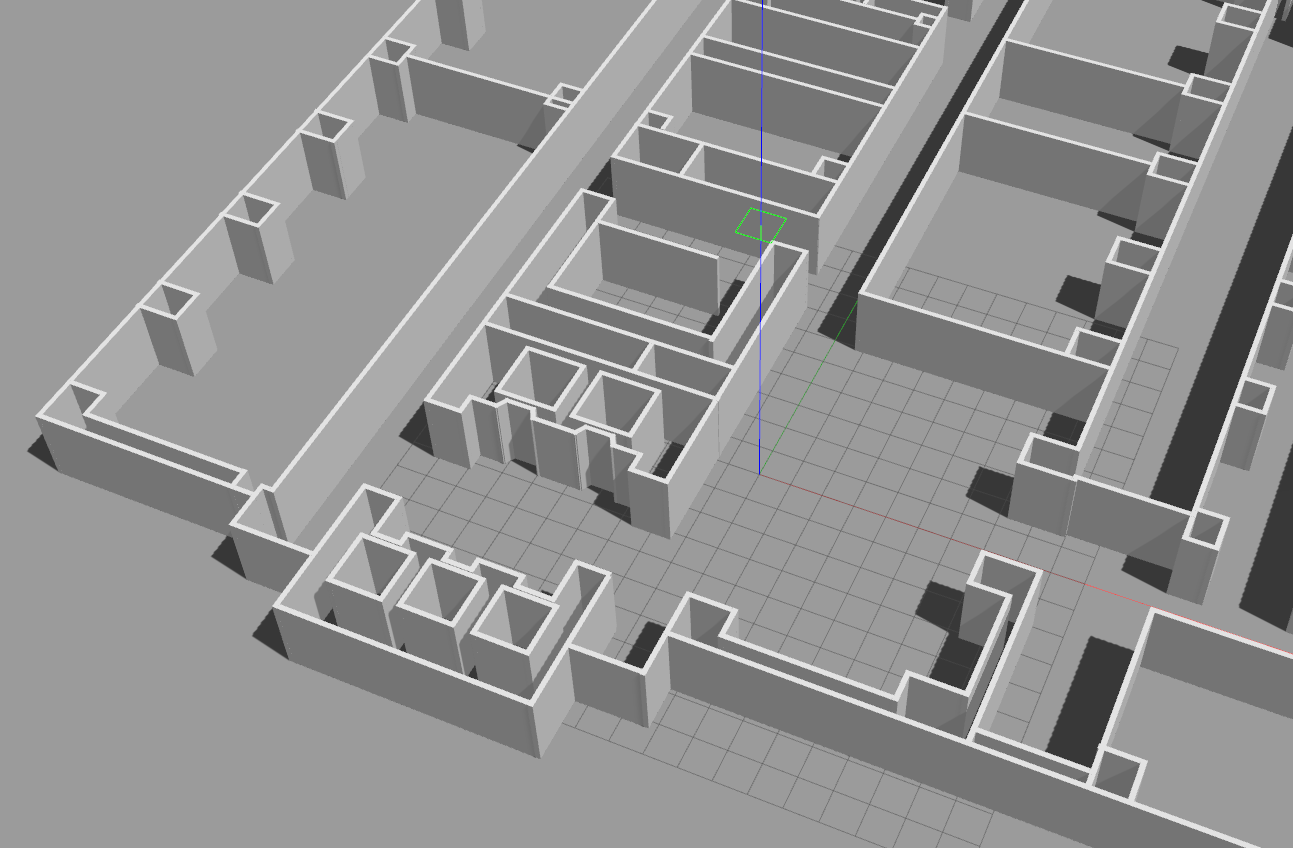
\includegraphics[keepaspectratio, scale=0.15]
      {images/sim-env.png}
\caption{Simulator Environment}
 \label{Fig:sim-env}
\end{figure} 

\vspace{-10pt}

\begin{figure}[H]
  \centering
  \begin{subfigure}{0.40\textwidth}
    \centering
    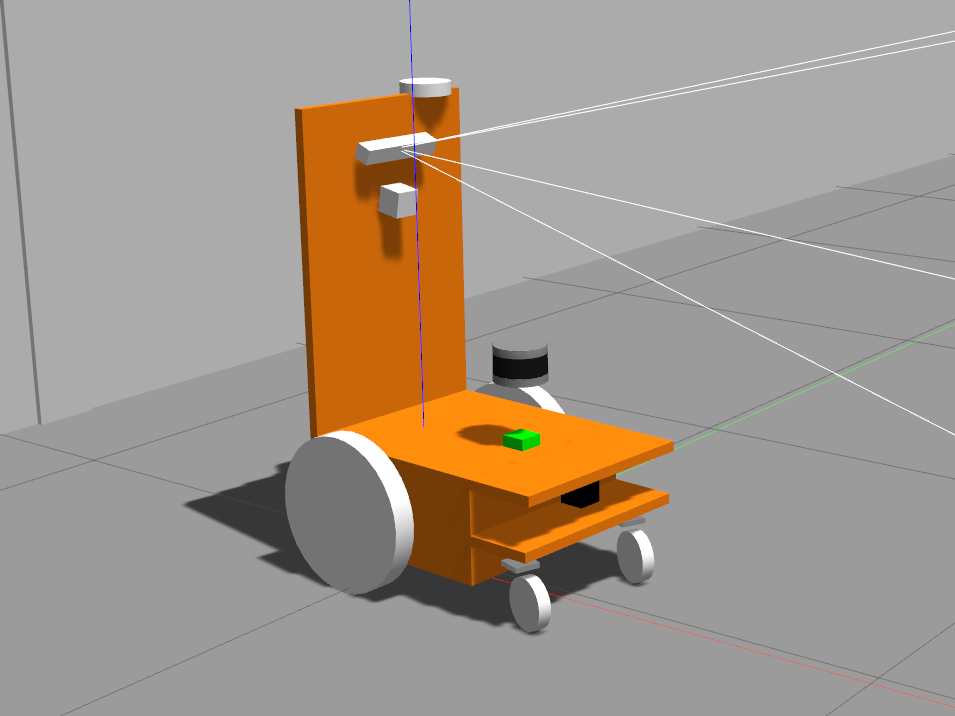
\includegraphics[keepaspectratio, scale=0.15]{images/sim-robot.png}
    \caption{Simulated Robot}
    \label{Fig:sim-robot}
  \end{subfigure}
  % \hfill
  \begin{subfigure}{0.40\textwidth}
    \centering
    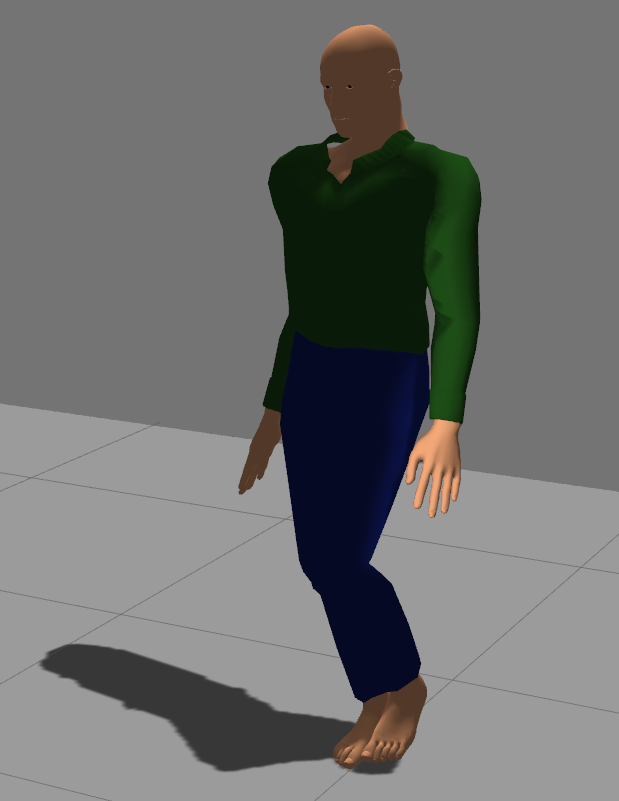
\includegraphics[keepaspectratio, scale=0.15]{images/sim-actor.png}
    \caption{Simulated Actor}
    \label{Fig:sim-actor}
  \end{subfigure}
  \caption{Simulated Robot and Actor}
  \label{Fig:sim-robot-actor}
\end{figure}

移動ロボットの自律走行は,つくばチャレンジ2024EX@イーアスつくば\cite{つくばチャレンジ36:online}で千葉工業大学 未来ロボティクス学科 box2チームが完走した際のソフトウェア構成,パラメータを参考にした.これは,Githubで公開されている\cite{openrdco85:online}.なお,後述するシナリオには狭い通路の走行が含まれるため,yaw方向の角速度を小さくなるように変更している.

\newpage

実験は\figref{Fig:experiment-scenarios}に示す2種類のシナリオで行った.
\figref{Fig:scenario1}に示すシナリオ1では,ロボットが直線経路を進む際に,歩行者が横断する状況を設定した.\figref{Fig:scenario2}に示すシナリオ2では,ロボットが狭い通路を進む際に,2名の歩行者がすれ違う状況を設定した.

\begin{figure}[H]
  \centering
  \begin{subfigure}{0.80\textwidth}
    \centering
    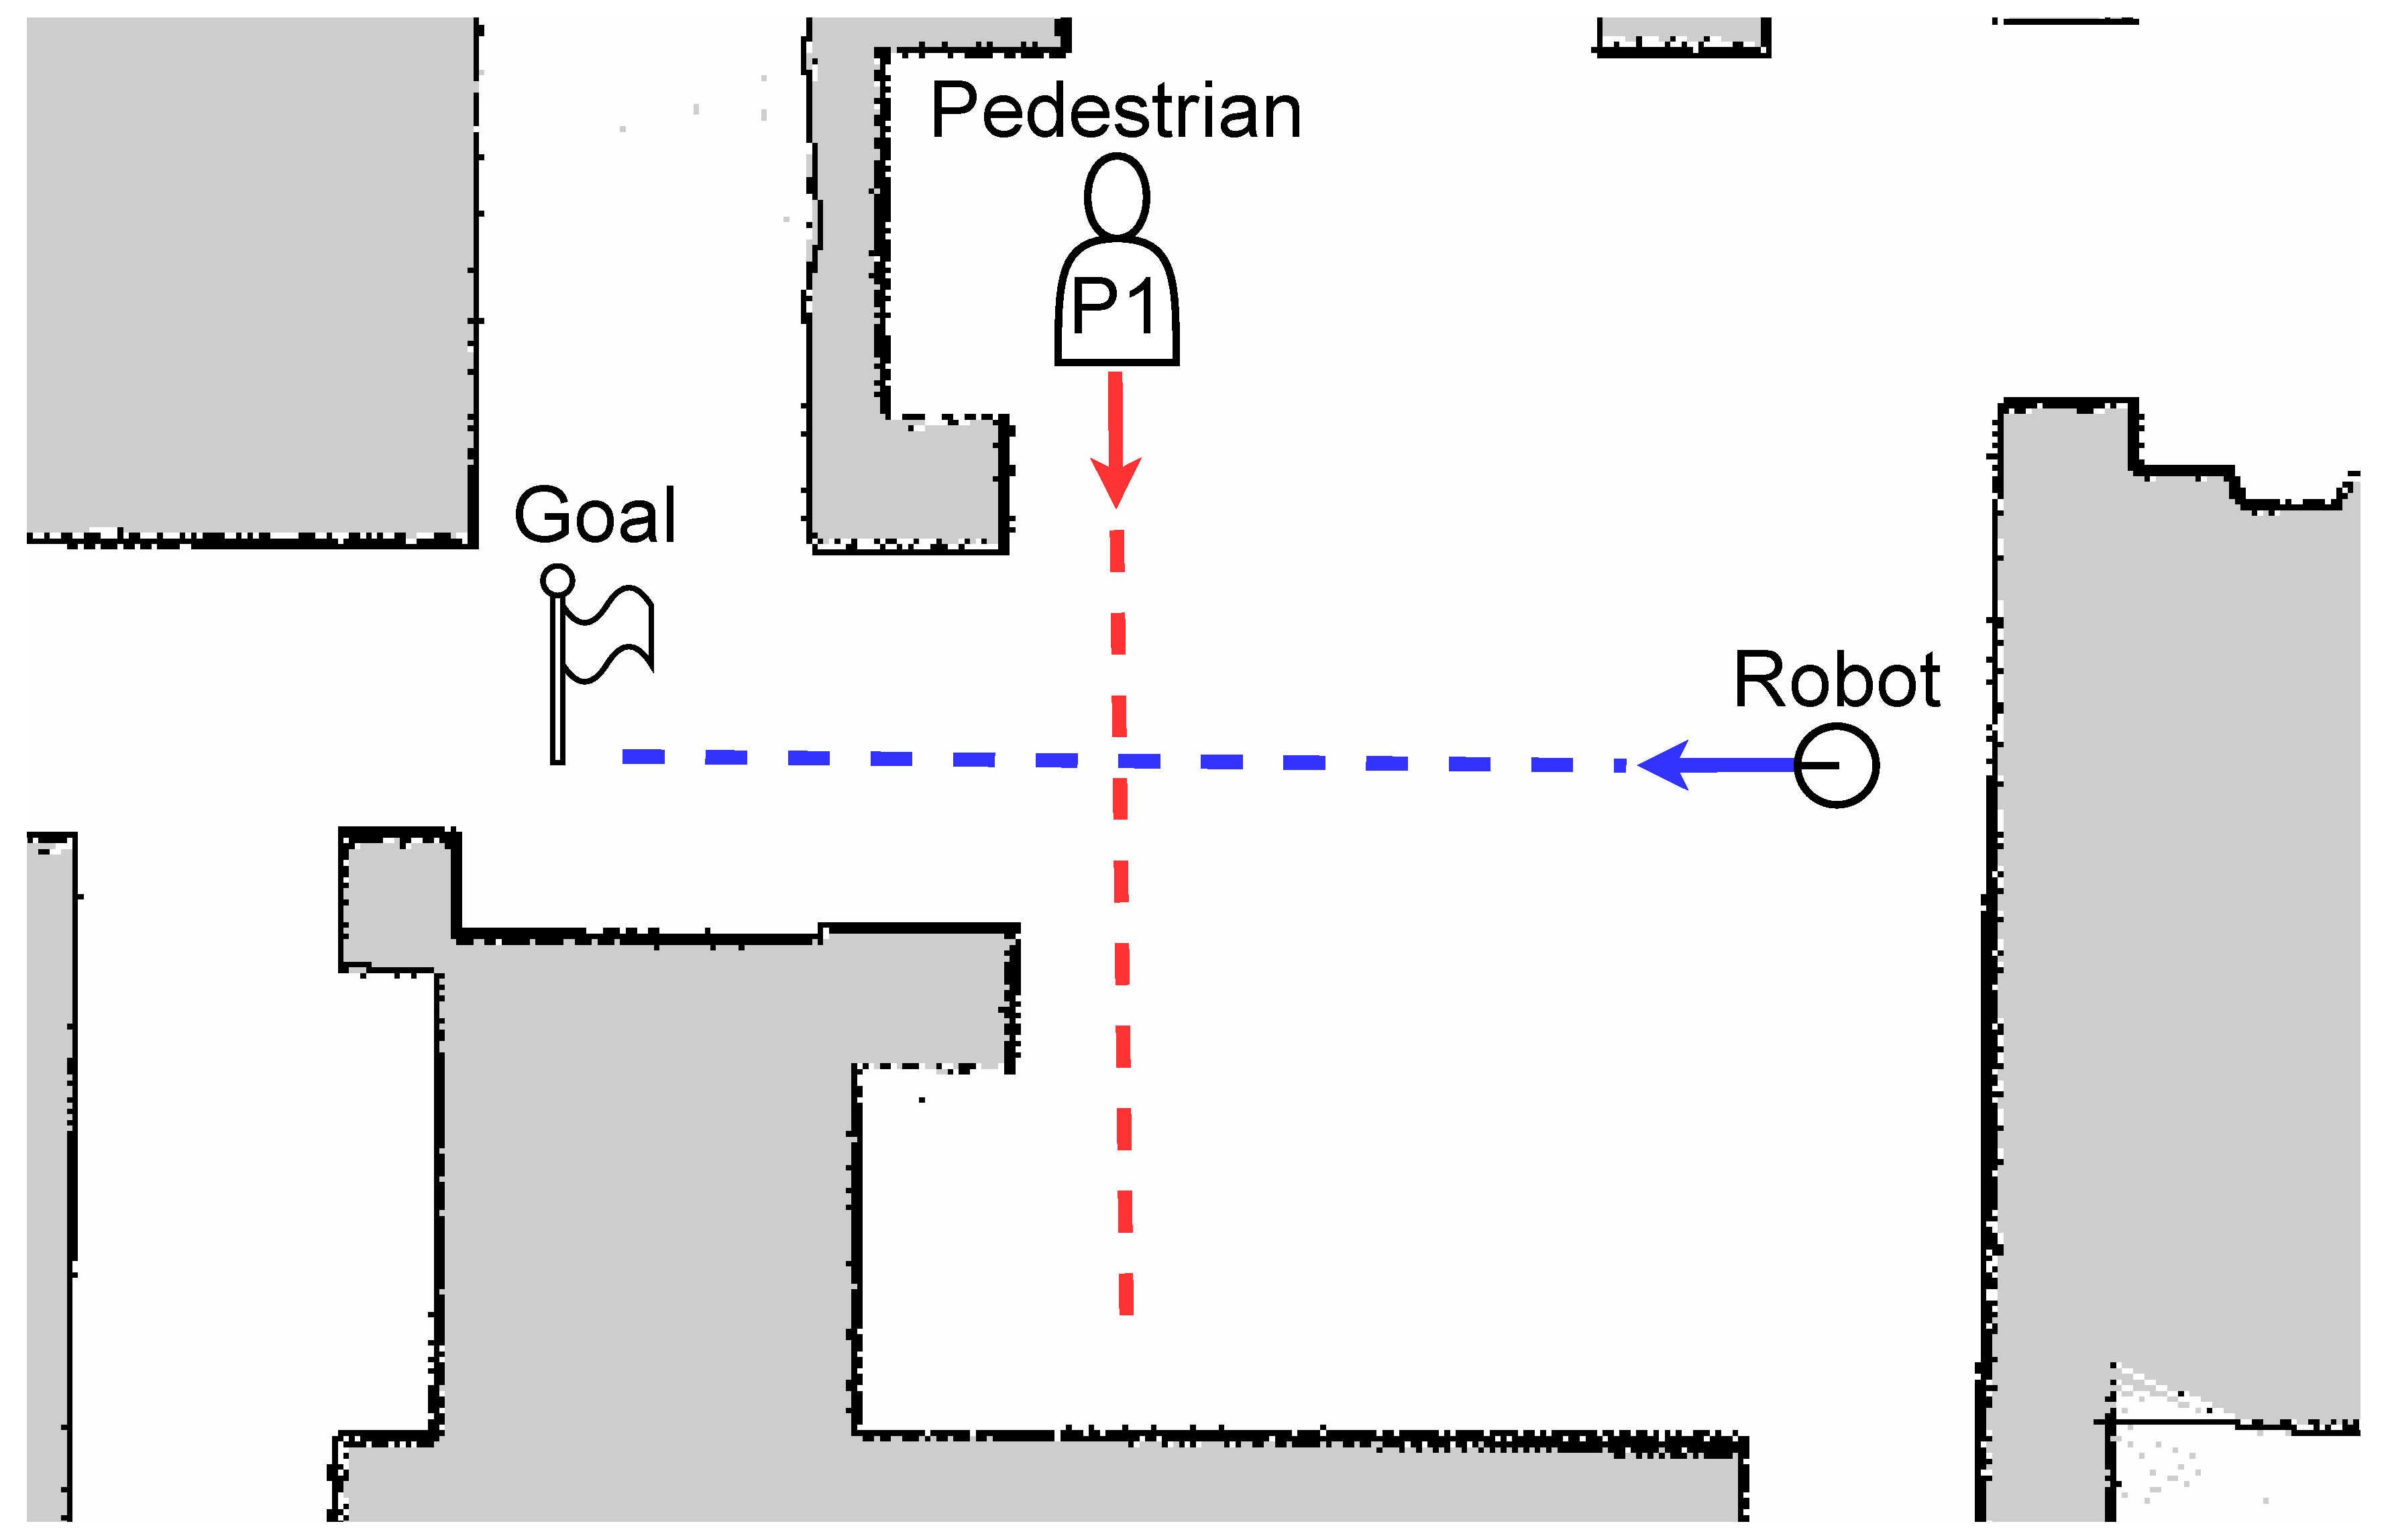
\includegraphics[keepaspectratio, scale=0.15]{images/scenario1.pdf}
    \caption{Scenario 1}
    \label{Fig:scenario1}
  \end{subfigure}
  \vspace{10pt}
  \begin{subfigure}{0.80\textwidth}
    \centering
    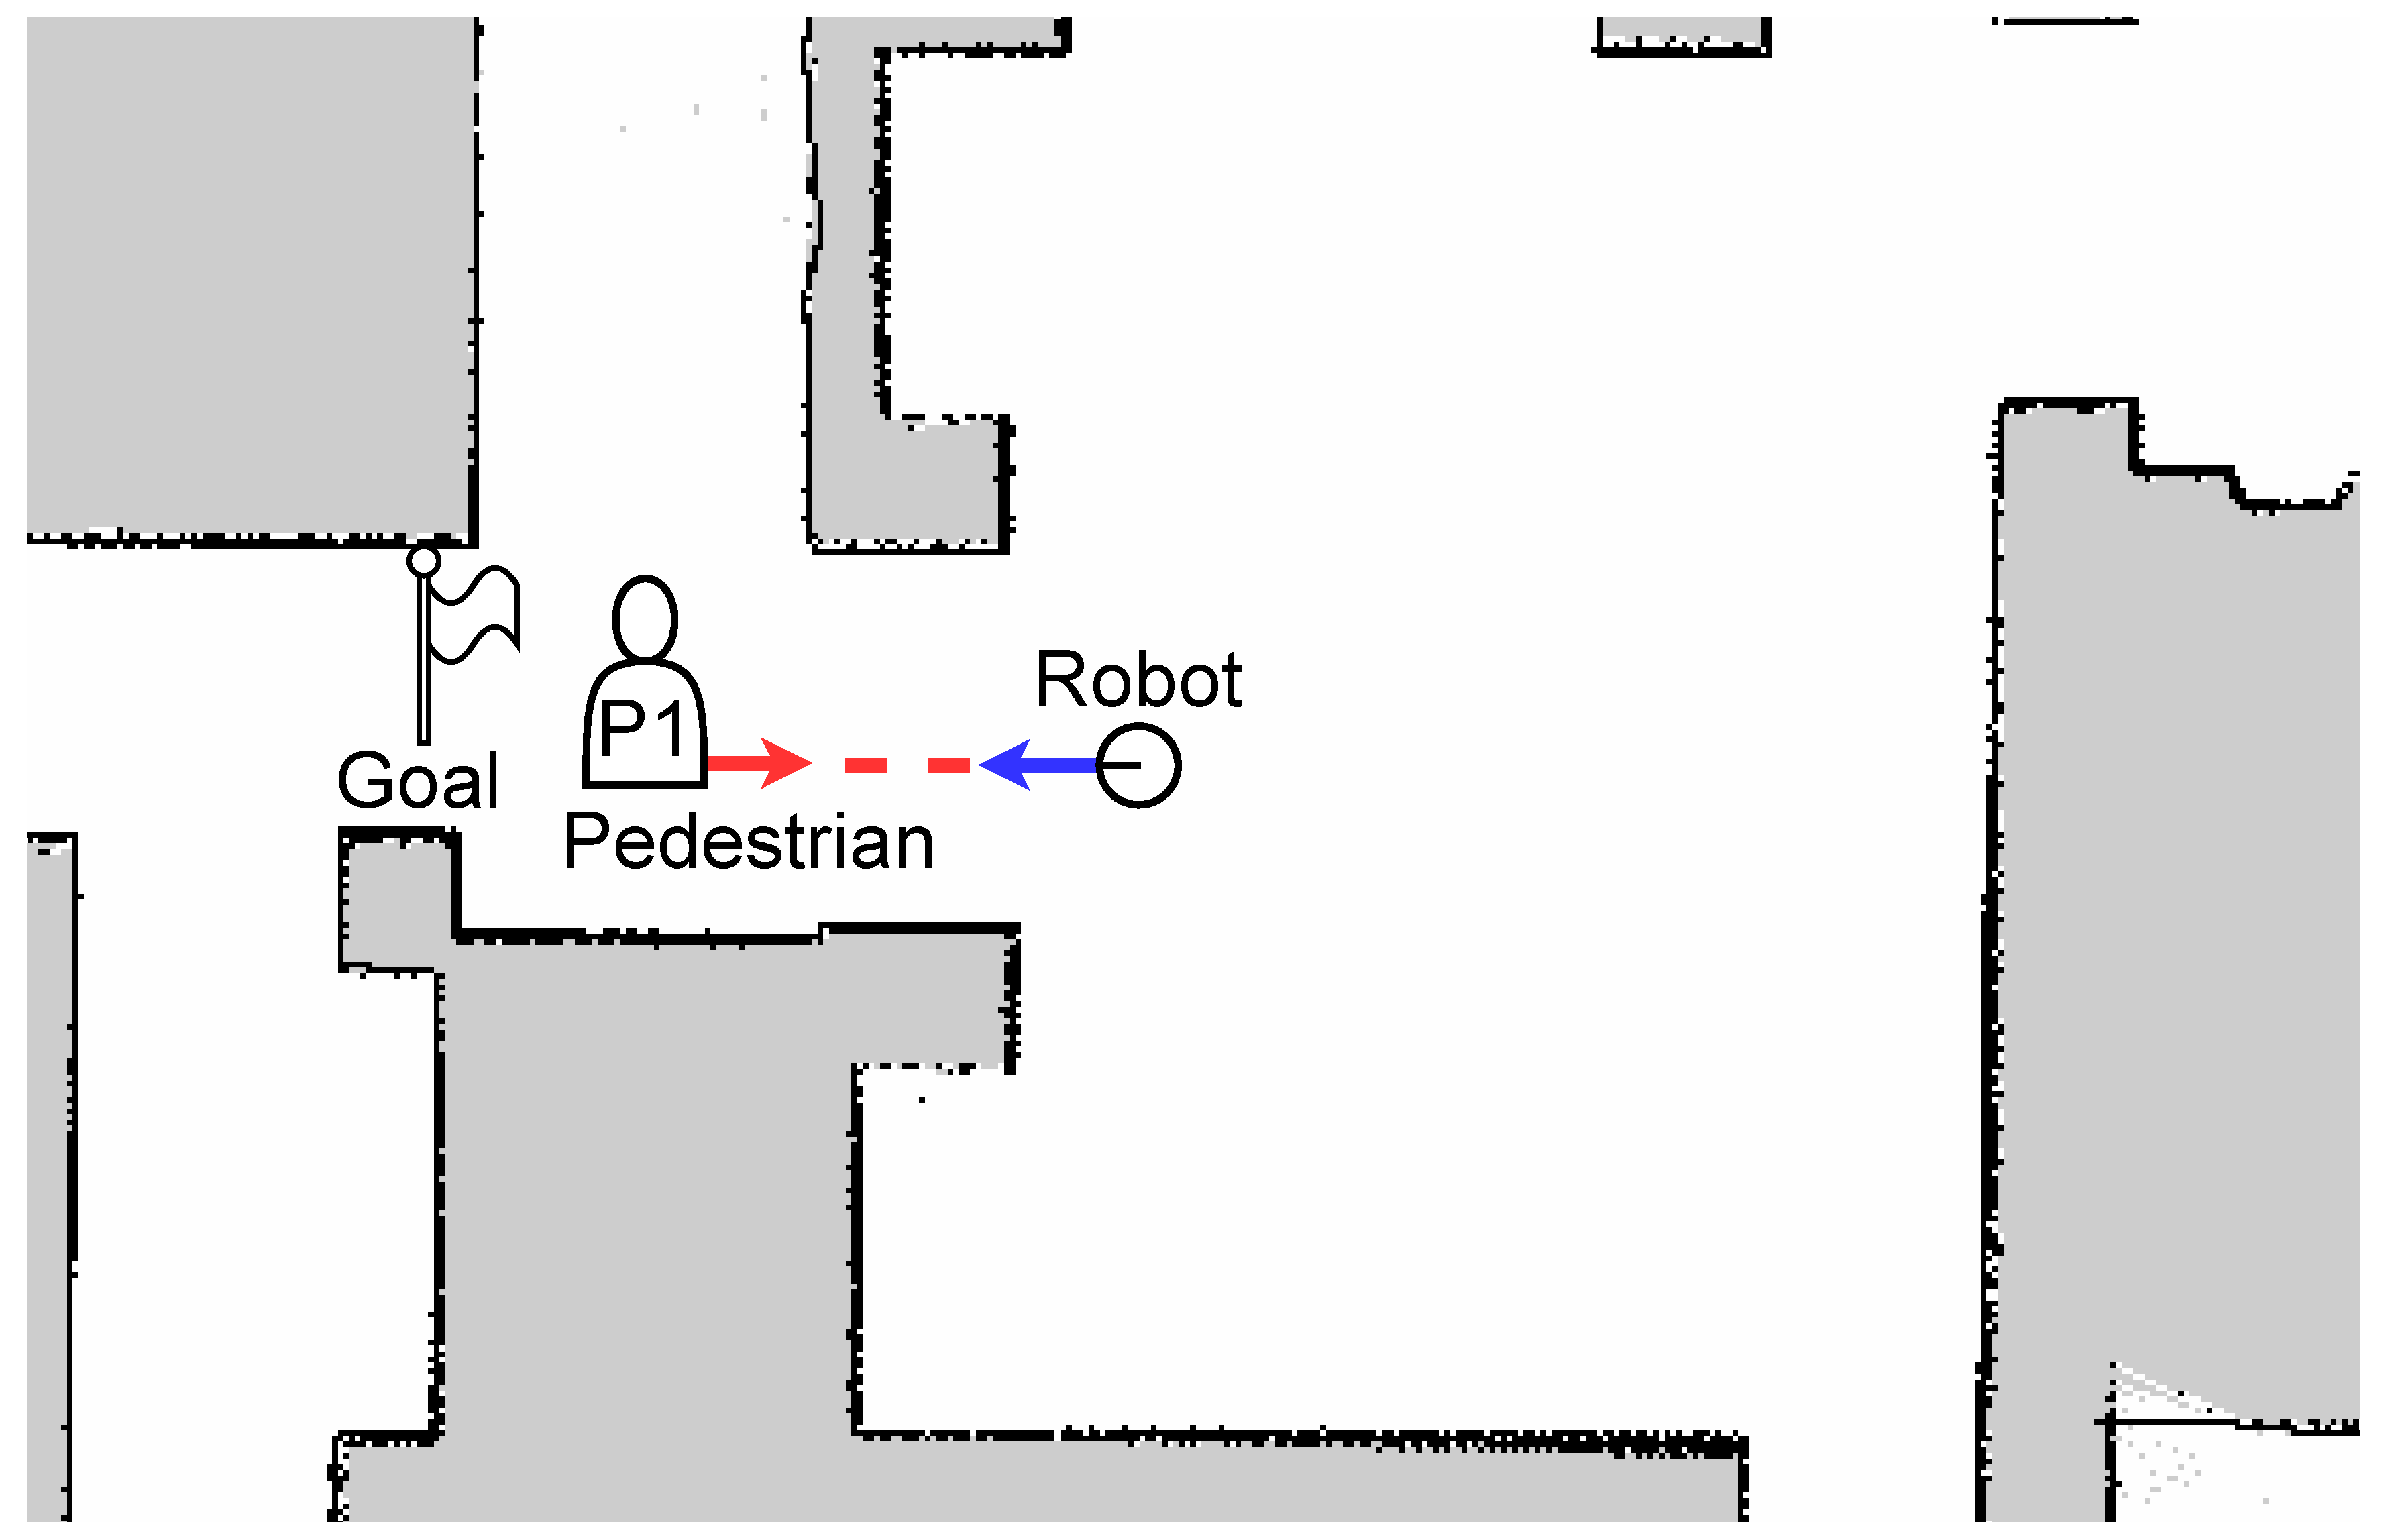
\includegraphics[keepaspectratio, scale=0.15]{images/scenario2.pdf}
    \caption{Scenario 2}
    \label{Fig:scenario2}
  \end{subfigure}
  \caption{Experiment Scenarios}
  \label{Fig:experiment-scenarios}
\end{figure}

\newpage

評価は以下の項目を基に行う.
\begin{itemize}
  \item 走行時間
  \item 走行距離
  \item 歩行者とロボット間の最小距離
  \item 最小のTime to Collision(TTC)
\end{itemize}
ナビゲーションは,走行時間と走行距離は小さいほど効率的であり,最小距離とTTCは大きいほど安全であると考えられる.
TTCは,移動する物体同士が現在の速度と進行方向を維持した場合に,衝突するまでの時間を示す指標であり,以下の式で計算される.
\setlength{\jot}{1em}
\begin{align}
  \mathbf{v}_{robot} = \begin{bmatrix} v_{robot,x} \\ v_{robot,y} \end{bmatrix}, \quad 
  \mathbf{v}_{ped} = \begin{bmatrix} v_{ped,x} \\ v_{ped,y} \end{bmatrix} \\
  \mathbf{v}_{relative} = \mathbf{v}_{robot} - \mathbf{v}_{ped} \\
  \text{TTC} = \frac{\text{d}}{\|\mathbf{v}_{relative}\|}
\end{align}
ここで,$d$はロボットと歩行者の距離,$\mathbf{v}_{robot}$はロボットの速度ベクトル,$\mathbf{v}_{ped}$は歩行者の速度ベクトルである.

\section{結果と考察}
\figref{Fig:scenario1-result},\figref{Fig:scenario2-result}に各シナリオにおいて,予測結果を用いないナビゲーションとロボットの行動を考慮した予測結果を用いるナビゲーションを比較した結果を示す.棒グラフは平均値,エラーバーは標準偏差を表している.
まず,\figref{Fig:scenario1-result}に示すシナリオ1の結果を比較すると,走行時間が約1.8倍,走行距離が約1.01倍と悪化した一方で,最小距離が約13倍,最小TTCが約17倍と大幅に改善した.
次に,\figref{Fig:scenario2-result}に示すシナリオ2の結果では,走行時間が約1.5倍,走行距離が約1.01倍,歩行者2の最小距離が0.9倍と悪化したが,歩行者1の最小距離が1.84倍,歩行者1の最小TTCが約1.3倍,歩行者2の最小TTCが約1.1倍と改善した.
これらの結果から,予測結果を用いることで,ロボットのナビゲーションがより安全になる可能性があることが示唆される.一方で,効率性の面では課題が残ることも確認された.

\begin{figure}[H]
  \centering
 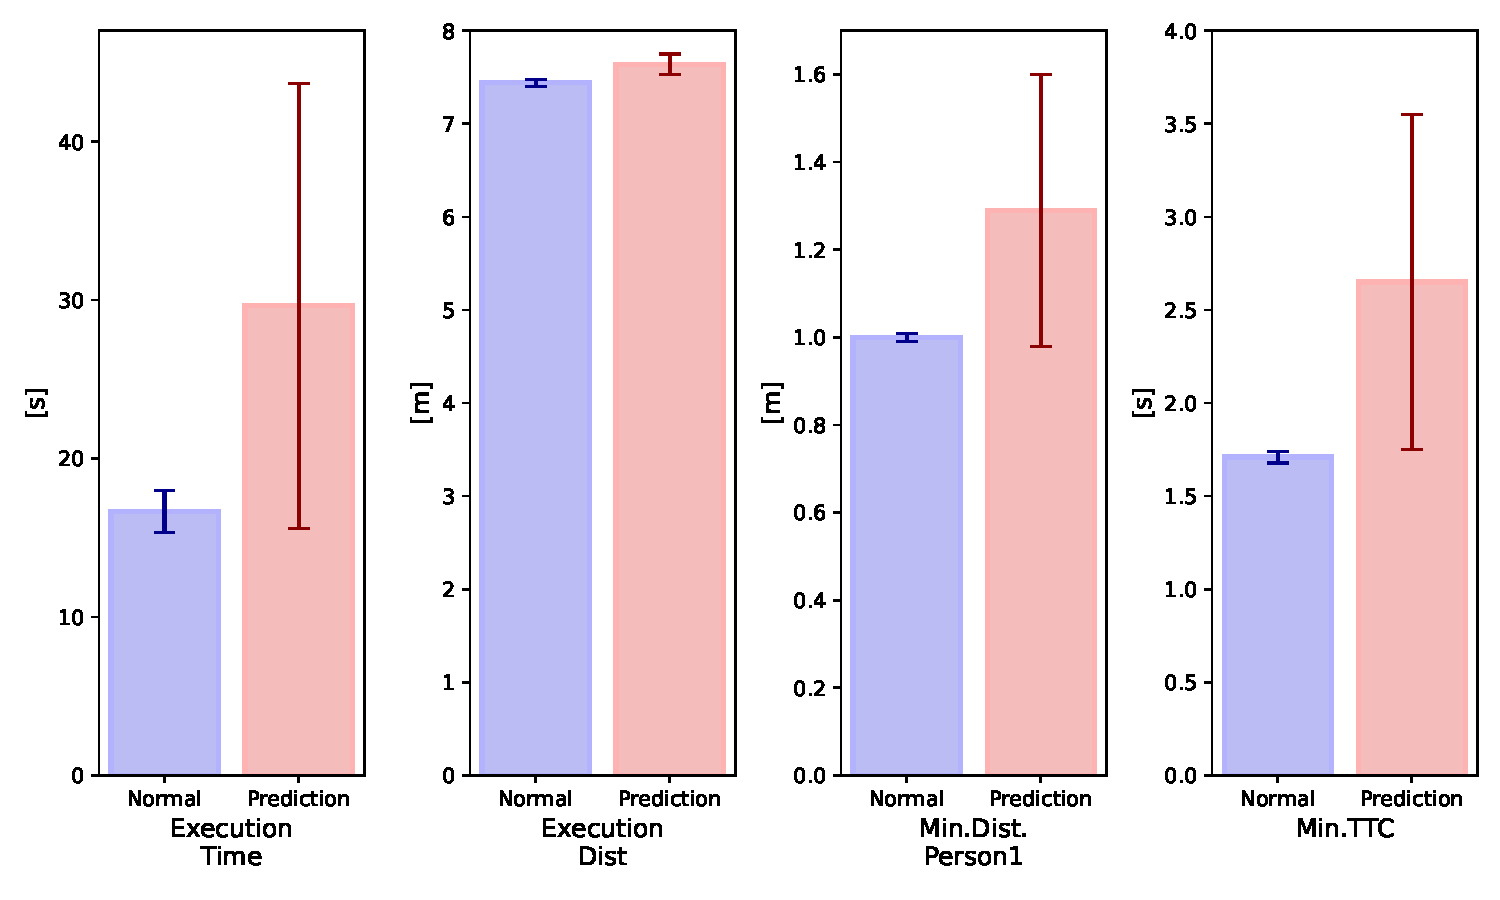
\includegraphics[keepaspectratio, scale=0.53]
      {images/scenario1_result.pdf}
  \caption{Scenario1 result}
 \label{Fig:scenario1-result}
\end{figure} 

\begin{figure}[H]
  \centering
 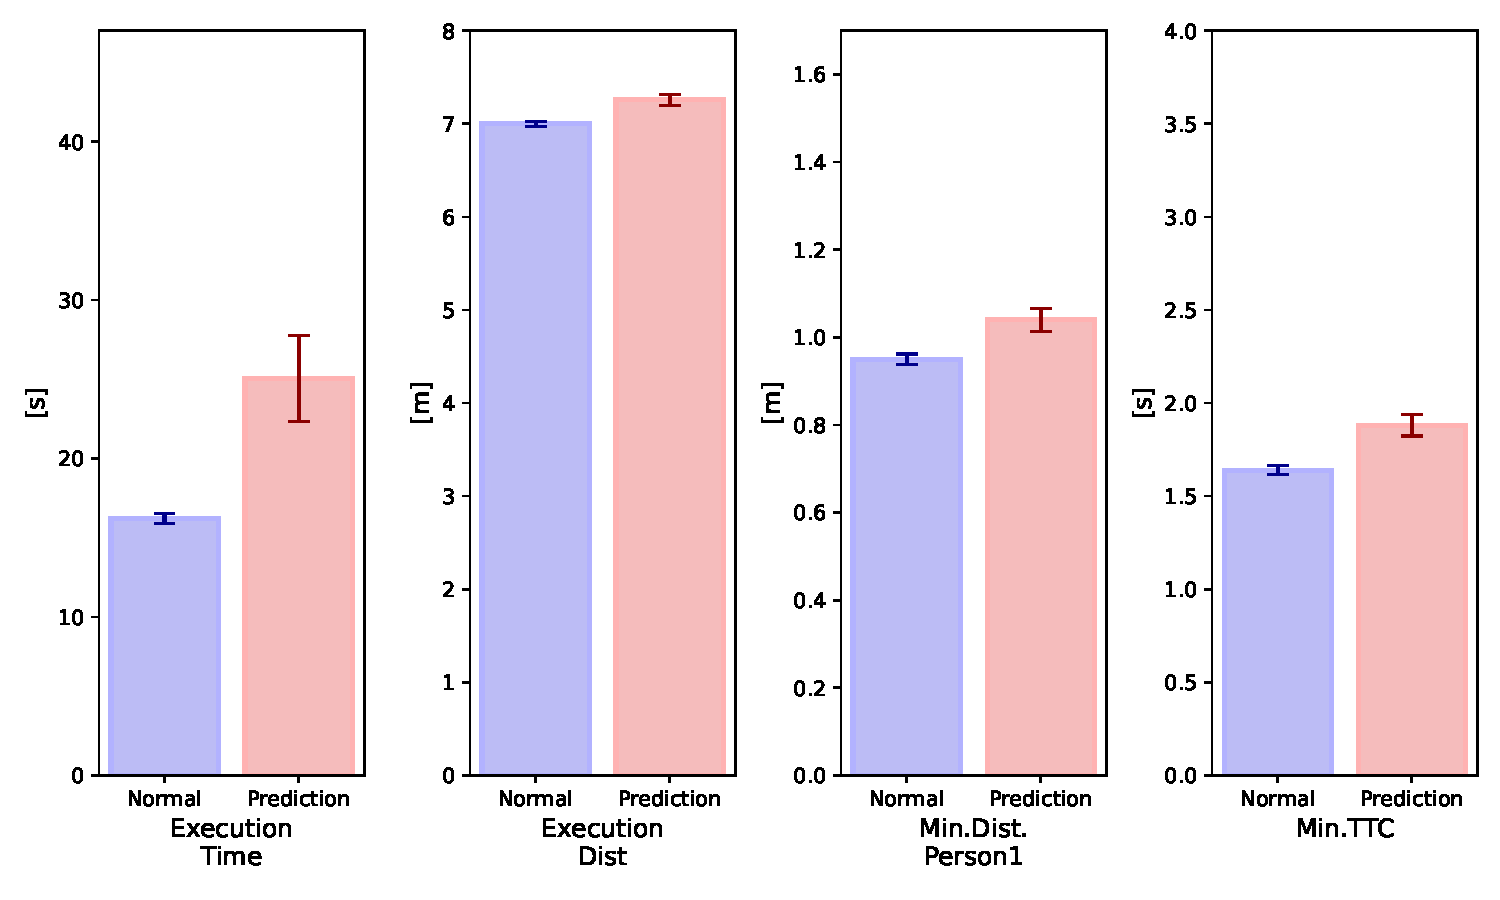
\includegraphics[keepaspectratio, scale=0.44]
      {images/scenario2_result.pdf}
  \caption{Scenario2 result}
 \label{Fig:scenario2-result}
\end{figure} 

シナリオ1では,歩行者との最小距離と最小TTCが大幅に改善されており,予測結果を用いることで早い段階で安全に停止することが確認できる.一方で,走行時間と走行距離が増加しているため,効率性の面では課題が残る.

シナリオ2では,歩行者1に対する最小距離と最小TTCが改善されているが,歩行者2に対する最小距離が悪化している.これは,狭い通路でのすれ違い時に,ロボットが歩行者2に対してより接近することを意味している.この結果から,狭い通路でのナビゲーションにおいては,予測結果の精度に改善の余地がある.これは,学習に用いたデータセットがいずれも屋外で広い空間のデータであるためだと考えられる.

本実験で用いたシミュレータの歩行者は,一定の線形軌道を常に同じ速度で歩行しており,現実の歩行者の動きとは大きく乖離している.つまり,歩行者同士や歩行者とロボット間など,全ての移動体の間に相互作用が存在しない.そのため,相互作用を重視して学習したデータと異なる環境であるため,予測性能が大幅に悪化している可能性がある.また,全体的に予測結果を用いた場合の評価項目における標準偏差が大きいと考えられる.他には,\ref{sec:nav-usage}節で述べたように,予測結果はガウス分布からサンプリングされた軌道を0.4秒ごとにコストマップに反映している.そのため,以下に示す要因も標準偏差を大きくしていると考えられる.
\begin{itemize}
  \item 実際の軌道とは大きく異なるものをサンプリングしてしまう
  \item 予測結果の反映周期が早いことによるロボットの経路計画のチャタリング
  \item $t-1\text{と}t$などの前後の予測結果に一貫性がない
\end{itemize}

\newpage
